\documentclass[12pt, twoside]{article}
\usepackage[letterpaper, margin=1in, headsep=0.2in]{geometry}
\setlength{\headheight}{0.6in}
%\usepackage[english]{babel}
\usepackage[utf8]{inputenc}
\usepackage{microtype}
\usepackage{amsmath}
\usepackage{amssymb}
%\usepackage{amsfonts}
\usepackage{siunitx} %units in math. eg 20\milli\meter
\usepackage{yhmath} % for arcs, overparenth command
\usepackage{tikz} %graphics
\usetikzlibrary{quotes, angles}
\usepackage{graphicx} %consider setting \graphicspath{{images/}}
\usepackage{parskip} %no paragraph indent
\usepackage{enumitem}
\usepackage{multicol}
\usepackage{venndiagram}

\usepackage{fancyhdr}
\pagestyle{fancy}
\fancyhf{}
\renewcommand{\headrulewidth}{0pt} % disable the underline of the header
\raggedbottom
\hfuzz=2mm %suppresses overfull box warnings

\usepackage{hyperref}

\fancyhead[LE]{\thepage}
\fancyhead[RO]{\thepage \\ Name: \hspace{4cm} \,\\}
\fancyhead[LO]{BECA / Dr. Huson / Geometry\\*  Unit 7: Geometry project\\* 5 December 2022}

\begin{document}

\subsubsection*{7.1 Homework: Review of analytic geometry}
\begin{enumerate}
  \item Graph and label the two equations. Mark their intersection as an ordered pair.
  \begin{multicols}{2}
    $y = \frac{1}{3}x+5$ \\
    $3x+2y = -12$
  \end{multicols}
  Are the lines parallel, perpendicular, or neither? Justify your answer.
  \vspace{1.5cm}
  \begin{center} %4 quadrant regents grid w T-Chart
  \begin{tikzpicture}[scale=.635]
    \draw [help lines] (-10,-10) grid (10,10);
    \draw [thick, ->] (-10.2,0) -- (10.4,0) node [below right] {$x$};
    \draw [thick, ->] (0,-10.2)--(0,10.4) node [left] {$y$};
  \end{tikzpicture}
  \end{center}

\item Find each value as a decimal rounded to three significant figures.
  \begin{enumerate}
    \begin{multicols}{2}
    \item   5.53581 \vspace{1cm}
    \item   24.34998
    \item   $5-\sqrt{3}$ \vspace{1cm}
    \item   $ 3 \pi$
    \end{multicols}
  \end{enumerate}
  \vspace{0.5cm}

\newpage
\item The line $l$ has the equation $y=-\frac{4}{3} x+7$.
\begin{enumerate}
  \item What is the slope of the line $k$, given $k \parallel l$?
  \vspace{1.5cm}
  \item What is the slope of the line $m$, given $m \perp l$?
  \vspace{1.5cm}
\end{enumerate}

\item On the graph below, draw $\overline{AB}$, with $A(1,5)$ and $B(5,-1)$, labeling the end points. Determine and state the coordinates of the midpoint $M$ of $\overline{AB}$ and mark and label it on the graph.
\begin{flushleft}
  \begin{tikzpicture}[scale=.635]
    \draw [help lines] (-3,-2) grid (8,7);
    \draw [thick, ->] (-3.2,0) -- (8.4,0) node [below right] {$x$};
    \draw [thick, ->] (0,-2.2)--(0,7.4) node [left] {$y$};
  \end{tikzpicture}
\end{flushleft}

\item Given $K(1,6)$ and $L(7,4)$, find the length of $\overline{KL}$, expressed as a simplified radical.\\[0.25cm]
Use: $l=\sqrt{(x_2-x_1)^2+(y_2-y_1)^2}$
    \vspace{4cm}

\newpage  
  \item Graph and label the two equations. Mark their intersection as an ordered pair.
  \begin{multicols}{2}
    $y = -x+8$ \\
    $3x-4y = -4$
  \end{multicols}
  Are the lines parallel, perpendicular, or neither? Justify your answer.
  \vspace{1.5cm}
  \begin{center} %4 quadrant regents grid w T-Chart
  \begin{tikzpicture}[scale=.635]
    \draw [help lines] (-10,-10) grid (10,10);
    \draw [thick, ->] (-10.2,0) -- (10.4,0) node [below right] {$x$};
    \draw [thick, ->] (0,-10.2)--(0,10.4) node [left] {$y$};
  \end{tikzpicture}
  \end{center}

\item Find each value as a decimal rounded to three significant figures.
  \begin{enumerate}
    \begin{multicols}{2}
    \item   1.73284 \vspace{1cm}
    \item   14.1578
    \item   $11-\sqrt{20}$ \vspace{1cm}
    \item   $ 2 \pi$
    \end{multicols}
  \end{enumerate}
  \vspace{0.5cm}

\newpage
\item The line $l$ has the equation $y=-\frac{2}{5} x+3$.
\begin{enumerate}
  \item What is the slope of the line $k$, given $k \parallel l$?
  \vspace{1.5cm}
  \item What is the slope of the line $m$, given $m \perp l$?
  \vspace{1.5cm}
\end{enumerate}

\item On the graph below, draw $\overline{AB}$, with $A(-1,2)$ and $B(7,6)$, labeling the end points. Determine and state the coordinates of the midpoint $M$ of $\overline{AB}$ and mark and label it on the graph.
\begin{flushleft}
  \begin{tikzpicture}[scale=.635]
    \draw [help lines] (-3,-2) grid (8,7);
    \draw [thick, ->] (-3.2,0) -- (8.4,0) node [below right] {$x$};
    \draw [thick, ->] (0,-2.2)--(0,7.4) node [left] {$y$};
  \end{tikzpicture}
\end{flushleft}

\item Given $K(1,6)$ and $L(-3,4)$, find the length of $\overline{KL}$, expressed as a simplified radical.\\[0.25cm]
Use: $l=\sqrt{(x_2-x_1)^2+(y_2-y_1)^2}$
    \vspace{4cm}

\newpage
\item A translation maps $A(1,12) \rightarrow A'(-3,2)$. What is the image of $B(10,-2)$ under the same translation?  \vspace{3cm}

In the following two problems, solve for the value of $x$.
\begin{multicols}{2}
  \item   $\frac{1}{5}(10x+5)=3$ \vspace{4cm}
  \item   $\frac{2}{3}(5-x)=-4$ \vspace{4cm}
  \end{multicols}
\vspace{4cm}

\item Given $f(x)=\frac{1}{3} x+3$. Solve for $x$ such that for $f(x)=2$. \vspace{4cm}
\item Given $g(x)=-2x^2-5x+3$. Simplify $g(1)$. \vspace{2cm}
%\item Given $h(x)=x^2-4x-5$. Solve $h(x)=0$. \vspace{3cm}

\newpage
\item In the diagram below, $\overline{AC}$ has endpoints with coordinates $A(-6,5)$ and $C(8, -2)$.
  \begin{center} %4 quadrant regents grid
    \begin{tikzpicture}[scale=.48]
      \draw [help lines] (-9,-5) grid (9,7);
      \draw [thick, <->] (-9.4,0) -- (9.4,0) node [below right] {$x$};
      \draw [thick, <->] (0,-5.4)--(0,7.4) node [left] {$y$};
      \draw [thick] (-6,5)--(8, -2);
      \draw [fill] (-6,5) circle [radius=0.1] node[above left] {$A$};
      \draw [fill] (8, -2) circle [radius=0.1] node[below right] {$C$};
    \end{tikzpicture}
  \end{center}
  If $B$ is a point on $\overline{AC}$ and $AB {:} BC = 2{:}5$,  what  are  the coordinates of $B$? \vspace{4cm}
  
\item $A(1,-3)$ is one endpoint of $\overline{AB}$. The segment's midpoint is $M(5,4)$. Find the other endpoint, $B$. \vspace{3cm}

\newpage
\item Spicy: Shown below is the quadrilateral $ABCD$ having coordinates $A(-3,-3)$, $B(5,1)$, $C(6,8)$, and $D(-2,4)$.
  \begin{center} %4 quadrant regents grid
  \begin{tikzpicture}[scale=.48]
    \draw [help lines] (-9,-5) grid (9,9);
    \draw [thick, <->] (-9.4,0) -- (9.4,0) node [below right] {$x$};
    \draw [thick, <->] (0,-5.4)--(0,9.4) node [left] {$y$};
    \draw [thick] (-3,-3) node[below] {$A$}--
    (5,1) node[right] {$B$}--
    (6,8) node[right] {$C$}--
    (-2,4) node[left] {$D$}--cycle;
    %\draw [fill] (5,0) circle [radius=0.1] node[above left] {$P$};
  \end{tikzpicture}
  \end{center}
  Given that $\overline{AD} \parallel \overline{BC}$. 
  \begin{enumerate}[itemsep=2cm]
    \item Find the slopes of $\overline{AB}$ and $\overline{CD}$\vspace{2cm}
    \item Hence, show that $\overline{AB} \parallel \overline{CD}$
    \item Use the definition that a parallelogram is a quadrilateral with two pairs of parallel sides to prove $ABCD$ is a parallelogram.
  \end{enumerate}


  
\end{enumerate}
\end{document}